\documentclass[aspectratio=169]{beamer}

\usepackage[T1]{fontenc}
\usepackage{lmodern}
\usepackage{amsmath,amssymb}
\usepackage{booktabs}
\usepackage{tabularx}
\usepackage{tikz}
\usetikzlibrary{arrows.meta,backgrounds,calc,positioning,shapes.multipart,fit}
\usepackage{ragged2e}
\usepackage{csquotes}
\usepackage[
  backend=biber,
  style=authoryear,
  maxcitenames=2,
  doi=false,
  isbn=false,
  url=true
]{biblatex}
\addbibresource{refs.bib}
% printbibliography resets font size per entry internally, so a plain \footnotesize
% wrapped around it in the slide has no effect — biblatex's own \bibfont hook is the
% only thing that actually controls bibliography-entry size.
\renewcommand*{\bibfont}{\footnotesize}

\definecolor{detectBlue}{HTML}{2D6CDF}
\usetheme[
  accent=detectBlue,
  progressbar=foot,
  sectionpage=none,
  subsectionpage=none,
  numbering=fraction,
  numberrail=subsection,
  block=fill,
  notes=hide,
  toc=none,
  closing=contact
]{cookie}

\setbeamerfont{title}{size=\fontsize{25}{28}}

% -----------------------------------------------------------------------------
% Title metadata — fill in the [TODO] fields before the final build.
% -----------------------------------------------------------------------------
\title[AI Image \& Alteration Detection]{AI-Generated Image \& Alteration Detection}
\subtitle{Two-Stream Spatial--Frequency Network}
\author[]{Francesco Innocenzi 2087246\\{}Luca Festugato 2064594}
\date{July 10th 2026}
\cookietagline{Project 2 \textbullet\ Real-World Scenarios}
\cookietitleimage{assets/intro.png}
\cookieclosingtitle{Thank You}
\cookieclosingtext{Questions \& Discussion}

% -----------------------------------------------------------------------------
% The theme's default title art sizes the background image by HEIGHT and
% anchors it narrowly, which leaves the accent-colored wedge showing at its
% wider (bottom) edge for portrait images. Override to size by WIDTH instead,
% wide enough to cover the wedge at its widest point, so the photo fills the
% whole shape with no blue showing through.
% -----------------------------------------------------------------------------
\makeatletter
\renewcommand{\cookie@drawtitleart}{%
  \begin{tikzpicture}[remember picture,overlay]
    \coordinate (cookie@cuttop) at ($(current page.north east)+(-.31\paperwidth,0)$);
    \coordinate (cookie@cutbottom) at ($(current page.south east)+(-.43\paperwidth,0)$);
    \path[fill=cookieAccent]
      (cookie@cuttop) -- (current page.north east) -- (current page.south east) -- (cookie@cutbottom) -- cycle;
    \ifdefempty{\insertcookiebackground}{%
      \draw[white,opacity=.18,line width=4pt] ($(current page.center)+(.34\paperwidth,.10\paperheight)$) circle[radius=.115\paperheight];
      \draw[white,opacity=.12,line width=3pt] ($(current page.center)+(.27\paperwidth,-.15\paperheight)$) circle[radius=.072\paperheight];
      \fill[white,opacity=.18] ($(current page.center)+(.40\paperwidth,-.22\paperheight)$) circle[radius=.018\paperheight];
      \fill[white,opacity=.22] ($(current page.center)+(.34\paperwidth,.26\paperheight)$) circle[radius=.012\paperheight];
    }{%
      \begin{scope}
        \clip (cookie@cuttop) -- (current page.north east) -- (current page.south east) -- (cookie@cutbottom) -- cycle;
        \node[anchor=center,inner sep=0] at ($(current page.east)+(-.20\paperwidth,0)$)
          {\includegraphics[width=.55\paperwidth]{\insertcookiebackground}};
        \fill[cookieAccent,opacity=.007] (current page.south west) rectangle (current page.north east);
      \end{scope}
    }%
    \ifx\inserttitlegraphic\@empty\else
      \node[anchor=center] at ($(current page.east)+(-.16\paperwidth,0)$) {\inserttitlegraphic};
    \fi
  \end{tikzpicture}%
}
\makeatother

% -----------------------------------------------------------------------------
% Placeholder box for figures that require running main.ipynb to generate
% (confusion matrices, ablation plots, GradCAM grids, ...). Keeps the deck
% compiling before those assets exist; swap for \includegraphics once produced.
% -----------------------------------------------------------------------------
\newcommand{\pendingfigure}[2][3.1cm]{%
  \begin{center}
    \begin{tikzpicture}
      \node[
        draw=cookieMuted,
        densely dashed,
        line width=.9pt,
        rounded corners=2pt,
        minimum width=.96\linewidth,
        minimum height=#1,
        align=center,
        text width=.80\linewidth,
        font=\small\itshape,
        text=cookieMuted
      ] {#2};
    \end{tikzpicture}
  \end{center}
}

\begin{document}

\input{slides/00_title.tex}
\begin{frame}{Outline}
  \begin{columns}[T,onlytextwidth]
    \column{.48\textwidth}
      \tableofcontents[hideallsubsections,sections={1-4}]
    \column{.48\textwidth}
      \tableofcontents[hideallsubsections,sections={5-8}]
  \end{columns}
\end{frame}

\section{Problem Statement}

\begin{frame}{The Challenge}
  \begin{columns}[T,onlytextwidth]
    \column{.58\textwidth}
      \footnotesize
      \begin{itemize}
        \item AI-generated imagery is now visually indistinguishable from real photographs.
        \item Two entangled problems: \textbf{Authenticity} (real or fake?) and \textbf{Provenance} (re-transmitted or re-digitized?).
        \item Real-world detectors must survive this ``laundering'' pipeline of re-compression and re-digitization.
        \item We frame this as a \textbf{joint} problem: processing history changes what artifacts remain for authenticity.
      \end{itemize}

    \column{.38\textwidth}
      \centering
      \begin{tikzpicture}[
          node distance=5mm,
          box/.style={cookie node,minimum width=2.7cm,minimum height=.75cm,font=\scriptsize\bfseries,align=center},
          accentbox/.style={cookie accent node,minimum width=2.7cm,minimum height=.75cm,font=\scriptsize\bfseries,align=center}
        ]
        \node[box] (orig) {Original image};
        \node[box,below=of orig] (transfer) {Transfer /\\compression};
        \node[box,below=of transfer] (redigital) {Re-digitization};
        \node[accentbox,below=of redigital] (detector) {Detector};
        \draw[cookie arrow] (orig) -- (transfer);
        \draw[cookie arrow] (transfer) -- (redigital);
        \draw[cookie arrow] (redigital) -- (detector);
      \end{tikzpicture}
  \end{columns}
\end{frame}

\section{State of the Art}

\begin{frame}{How Others Approach This}
  \begin{columns}[T,onlytextwidth]
    \column{.60\textwidth}
      \footnotesize
      \begin{itemize}
        \item \textbf{Spatial CNN detectors} (e.g.\ Xception on FaceForensics++ \cite{rossler2019faceforensics}) — learn texture artifacts from RGB; strong in-domain, weak on unseen generators.
        \item \textbf{Frequency-domain detectors} — GAN/diffusion upsampling leaves spectral peaks \cite{durall2020watch,frank2020leveraging}; often more compression-robust.
        \item \textbf{Generalization, not in-domain accuracy}, is the real bottleneck \cite{wang2020cnngenerated}.
        \item \textbf{Multi-task learning} — auxiliary labels regularize the shared representation \cite{kendall2018multitask}.
        \item \textbf{Gap this project targets:} benchmarks rarely treat re-digitization as its own task.
      \end{itemize}

    \column{.36\textwidth}
      \centering\scriptsize
      \begin{tabularx}{\linewidth}{@{}lcc@{}}
        \toprule
        Method & Comp. & Prov. \\
        \midrule
        Spatial    & \cookiecross & \cookiecross \\
        Frequency  & \cookiecheck & \cookiecross \\
        Multi-task & \cookiecheck & \cookiecross \\
        \textbf{Ours} & \cookiecheck & \cookiecheck \\
        \bottomrule
      \end{tabularx}
      \vspace{.4em}
      {\tiny\color{cookieMuted} Comp.\ = robust to compression; Prov.\ = models provenance}
  \end{columns}
\end{frame}

\section{Proposed Method}
\subsection{Architecture}

\begin{frame}{Two-Stream Multi-Task Network}
  \begin{columns}[T,onlytextwidth]
    \column{.46\textwidth}
      \footnotesize
      \begin{itemize}
        \item Two parallel feature extractors, fused before two heads:
        \begin{itemize}
          \item \textbf{Spatial branch}: pretrained backbone (ResNet-50/ConvNeXt) — texture cues.
          \item \textbf{Frequency branch}: lightweight CNN on the FFT — spectral fingerprints.
        \end{itemize}
        \item Concatenated features $\to$ two heads: \textbf{Real vs.\ Fake} (BCE), \textbf{Transform type} (3-class CE).
        \item Both heads use \textbf{both} branches — GradCAM later shows which one drives what.
      \end{itemize}

    \column{.50\textwidth}
      \centering
      \begin{tikzpicture}[
          box/.style={cookie node,minimum width=1.9cm,minimum height=.65cm,font=\tiny\bfseries,align=center},
          accentbox/.style={cookie accent node,minimum width=1.9cm,minimum height=.65cm,font=\tiny\bfseries,align=center}
        ]
        \node[box] (img) at (2.1,5.6) {Image};
        \node[box] (spatial) at (0.3,4.1) {Spatial\\backbone};
        \node[box] (fft) at (3.9,4.1) {FFT};
        \node[box] (freq) at (3.9,2.6) {Frequency\\CNN};
        \node[accentbox] (concat) at (2.1,1.5) {Concat};
        \node[box] (head1) at (0.3,0.1) {Head 1:\\Real/Fake};
        \node[box] (head2) at (3.9,0.1) {Head 2:\\Transform};

        \draw[cookie arrow] (img) -- (spatial);
        \draw[cookie arrow] (img) -- (fft);
        \draw[cookie arrow] (fft) -- (freq);
        \draw[cookie arrow] (spatial) -- (concat);
        \draw[cookie arrow] (freq) -- (concat);
        \draw[cookie arrow] (concat) -- (head1);
        \draw[cookie arrow] (concat) -- (head2);
      \end{tikzpicture}
  \end{columns}
\end{frame}

\subsection{Frequency Branch}

\begin{frame}{Why Add a Frequency Branch?}
  \begin{columns}[T,onlytextwidth]
    \column{.52\textwidth}
      \footnotesize
      \begin{itemize}
        \item Generative models (GANs especially) leave periodic upsampling artifacts, subtle spatially but visible as peaks/asymmetries in the Fourier spectrum.
        \item \textbf{Pipeline:} RGB $\to$ FFT2 $\to$ shift zero-frequency to center $\to$ log-magnitude + phase $\to$ per-channel min-max normalize to $[0,1]$ $\to$ 6-channel input $\to$ small 4-block CNN $\to$ 256-d feature.
        \item Kept lightweight (4 conv blocks, no pretrained backbone): this domain differs too much from ImageNet textures for transfer learning to help.
      \end{itemize}

    \column{.44\textwidth}
      \centering
      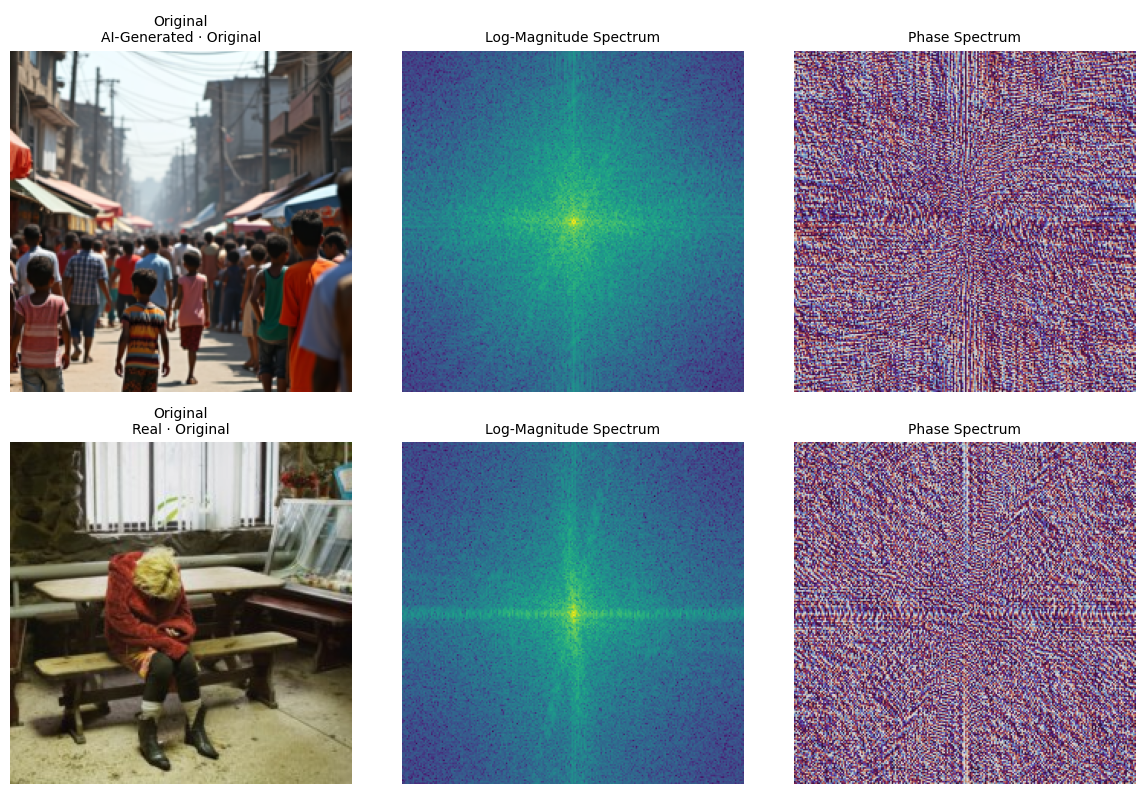
\includegraphics[width=\linewidth]{assets/frequency_spectrum_example.png}\\
      {\scriptsize\color{cookieMuted} RGB vs.\ FFT log-magnitude spectrum}
  \end{columns}
\end{frame}

\subsection{Training Strategy}

\begin{frame}{Multi-Task Loss \& Ablation}
  \footnotesize
  \setlength{\abovedisplayskip}{3pt}
  \setlength{\belowdisplayskip}{3pt}
  \begin{itemize}
    \item \textbf{Fixed weights} — manual $\alpha/\beta$ sweep (e.g.\ $0.5/0.5$):
    \[
      \mathcal{L} = \alpha \cdot \text{BCE}_{\text{RF}} + \beta \cdot \text{CE}_{\text{Transform}}
    \]
    \item \textbf{Uncertainty weighting} \cite{kendall2018multitask} — learnable per-task noise $\sigma_i$ auto-balances the loss:
    \[
      \mathcal{L}(\sigma_1,\sigma_2) = \frac{1}{2\sigma_1^{2}}\,\text{BCE}_{\text{RF}} + \frac{1}{2\sigma_2^{2}}\,\text{CE}_{\text{Transform}} + \log\sigma_1 + \log\sigma_2
    \]
    \item \textbf{Ablation engine}: one model per configuration, early stopping (patience 3), keeping only the \emph{best} epoch.
  \end{itemize}

  \begin{alertblock}{Anti-shortcut fix}
    \footnotesize Augmentation applied only to \texttt{transfer} images let the network detect compression instead of real signal (since \texttt{transfer}/\texttt{redigital} were \texttt{.jpg}, \texttt{original} was \texttt{.png}). Fixed by applying it uniformly across all classes.
  \end{alertblock}
\end{frame}

\section{Dataset}

\begin{frame}{Dataset}
  \begin{columns}[T,onlytextwidth]
    \column{.46\textwidth}
      \footnotesize
      \textbf{RRDataset} — $\sim$51{,}000 images across 3 processing categories $\times$ 2 classes:
      \vspace{.25em}
      \centering
      \begin{tabularx}{\linewidth}{@{}Xrr@{}}
        \toprule
        Category & AI & Real \\
        \midrule
        Original            & 8500 & 8500 \\
        Transfer            & 8500 & 8500 \\
        Re-digitized        & 8500 & 8499 \\
        \bottomrule
      \end{tabularx}

      \vspace{.35em}
      \raggedright
      \begin{itemize}
        \item Balanced sampling per class (default 6000/class), fixed seed.
        \item \textbf{Leakage-safe split}: images grouped by parent photo ID before the 80/10/10 split, so a processed photo never lands in a different split than its original.
        \item Labels: Real/Fake (\texttt{ai=0}, \texttt{real=1}), Transform (\texttt{original=0}, \texttt{transfer=1}, \texttt{redigital=2}).
      \end{itemize}

    \column{.50\textwidth}
      \centering
      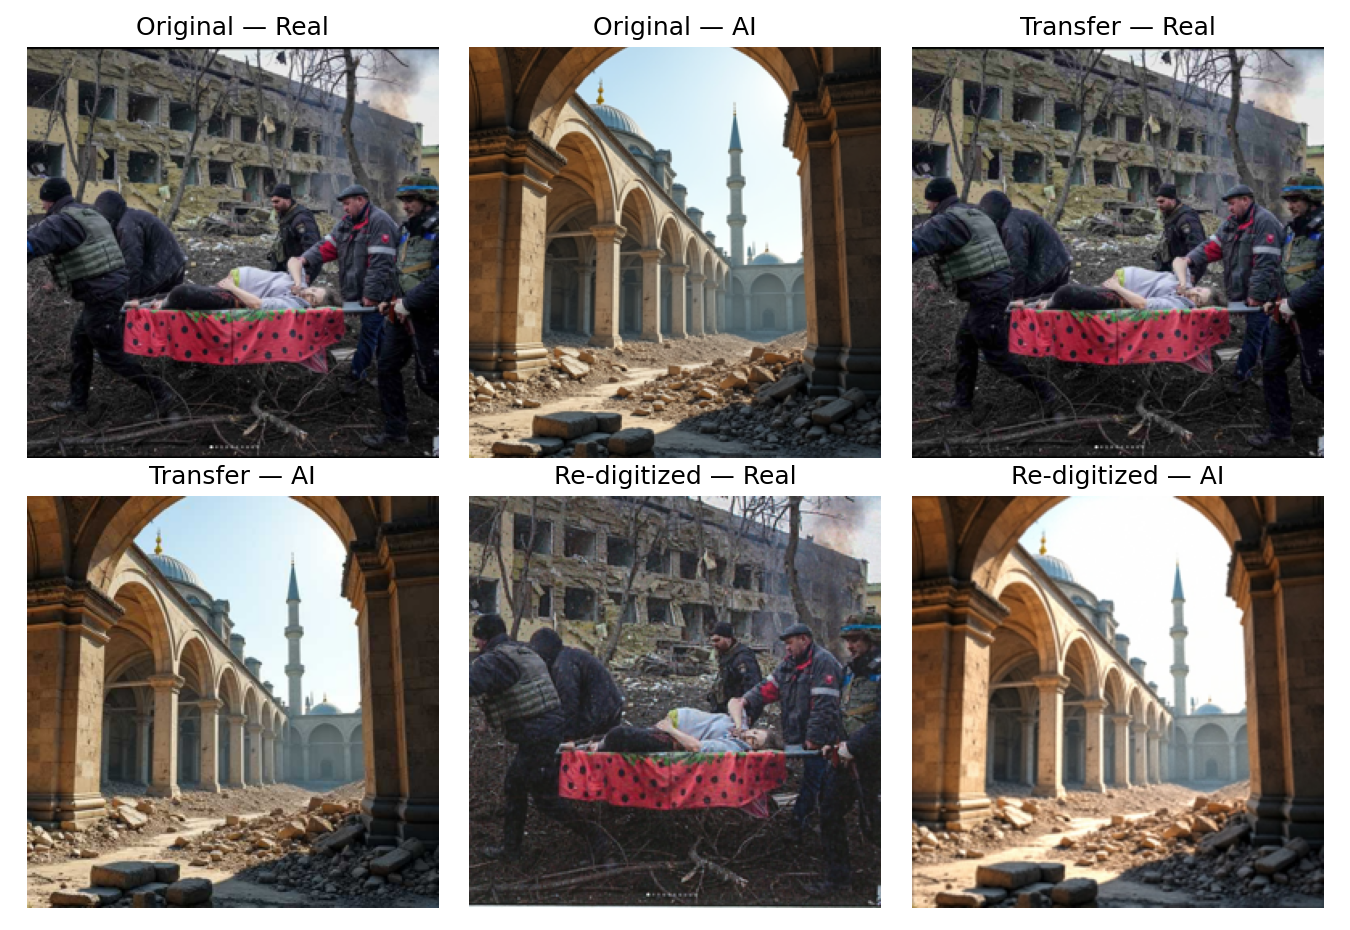
\includegraphics[width=\linewidth]{assets/dataset_samples.png}\\
      {\footnotesize\color{cookieMuted} One sample per (category $\times$ real/fake) cell}
  \end{columns}
\end{frame}

\section{Experimental Setup}

\begin{frame}{Experimental Setup}
  \centering\small
  \renewcommand{\arraystretch}{1.6}
  \begin{tabularx}{.92\textwidth}{@{}>{\bfseries}lX@{}}
    \toprule
    Setting & Value \\
    \midrule
    Backbones & ResNet-50 (23.9M), ConvNeXt-Tiny (28.2M) — ImageNet-pretrained \\
    Preprocessing & Resize 256 $\to$ crop 224 $\to$ ImageNet norm \\
    Augmentation (train) & H-flip; color jitter ($p{=}0.4$); light blur ($p{=}0.1$); JPEG re-compression (q30--95, $p{=}0.5$) — uniform across all classes \\
    Optimizer & Adam, LR $10^{-4}$ (ablation) \\
    Batch / epochs & 64, $\leq$10 epochs/config, early-stop patience 3 \\
    Configurations & 6/backbone: 5 fixed $\alpha/\beta$ + 1 uncertainty run \\
    Hardware & RTX 5070 Ti \\
    \bottomrule
  \end{tabularx}
\end{frame}

\section{Model Evaluation}
\subsection{Quantitative Results}

\begin{frame}{Results}
  \begin{itemize}
    \item Report on the held-out test set for the best checkpoint(s):
    \begin{itemize}
      \item Real/Fake: Accuracy, Precision, Recall, F1, ROC-AUC — \texttt{[TODO: run evaluate\_model() and fill in numbers]}
      \item Transform: Accuracy — \texttt{[TODO]}
    \end{itemize}
    \item Compare backbones side by side (ResNet-50 vs.\ ConvNeXt-Tiny vs.\ ConvNeXt-Base) on the same metrics.
    \item Compare fixed-weight vs.\ uncertainty-weighted loss.
  \end{itemize}

  \vspace{.4em}
  \begin{columns}[T,onlytextwidth]
    \column{.48\textwidth}
      \pendingfigure[2.6cm]{\texttt{confusion\_matrices.png}\\(both tasks)}
    \column{.48\textwidth}
      \pendingfigure[2.6cm]{\texttt{backbone\_comparison.png}\\(grouped bar chart across backbones)}
  \end{columns}
\end{frame}

\begin{frame}{Results — Backbone Comparison}
  \footnotesize
  \begin{itemize}
    \item Same test set, same evaluation code, best config per backbone — ConvNeXt-Tiny ahead on both tasks.
    \item Fixed weights slightly edge out learned uncertainty weighting on both backbones, but the gap is small — a reasonable no-tuning default.
  \end{itemize}

  \vspace{.3em}
  \centering
  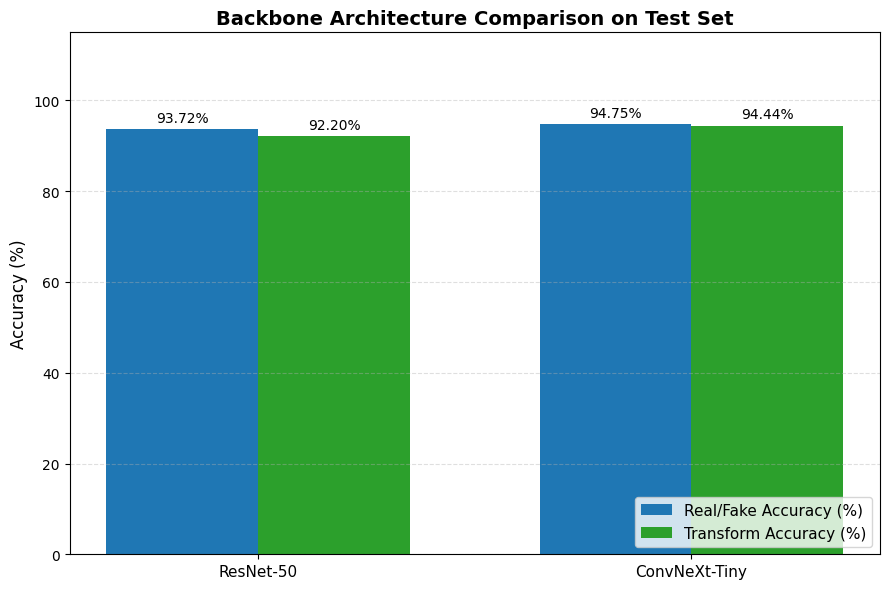
\includegraphics[height=4.6cm]{assets/backbone_comparison.png}
\end{frame}

\subsection{Robustness \& Calibration}

\begin{frame}{Robustness Across Processing Stages}
  \footnotesize
  \begin{itemize}
    \item Real/Fake accuracy \textbf{per transform category} (ConvNeXt-Tiny): weakest on Transmitted (90.8\%), strongest on Re-digitized (98.7\%) — Original/Transmitted is the main confusion pair on both backbones.
  \end{itemize}

  \vspace{.3em}
  \centering
  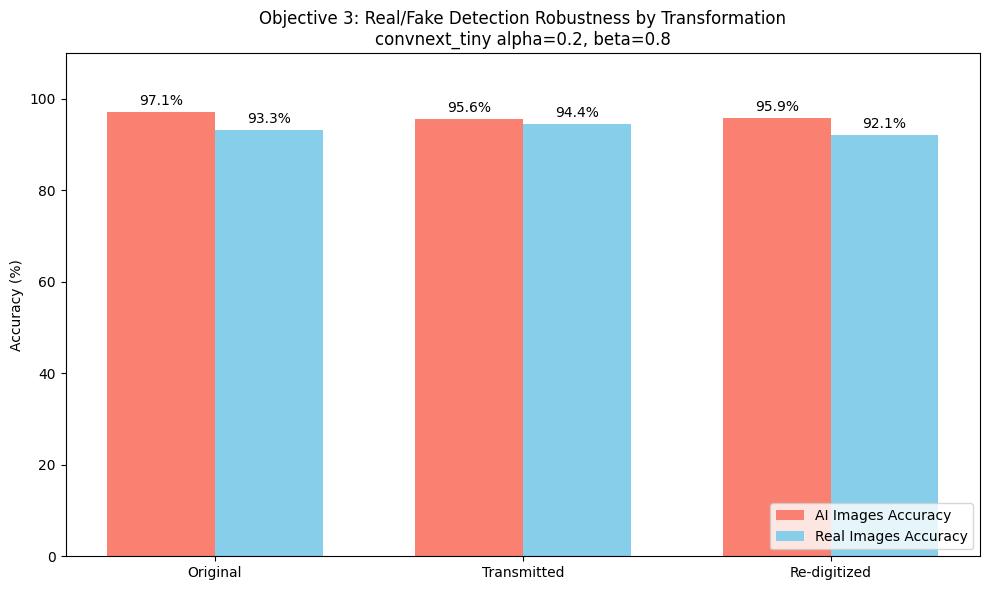
\includegraphics[height=5.1cm]{assets/accuracy_breakdown.png}
\end{frame}

\begin{frame}{Robustness — ROC \& Precision-Recall}
  \footnotesize
  \begin{itemize}
    \item ROC-AUC 0.989, near-perfect separation on the Real/Fake task (ConvNeXt-Tiny, best config).
  \end{itemize}

  \vspace{.3em}
  \centering
  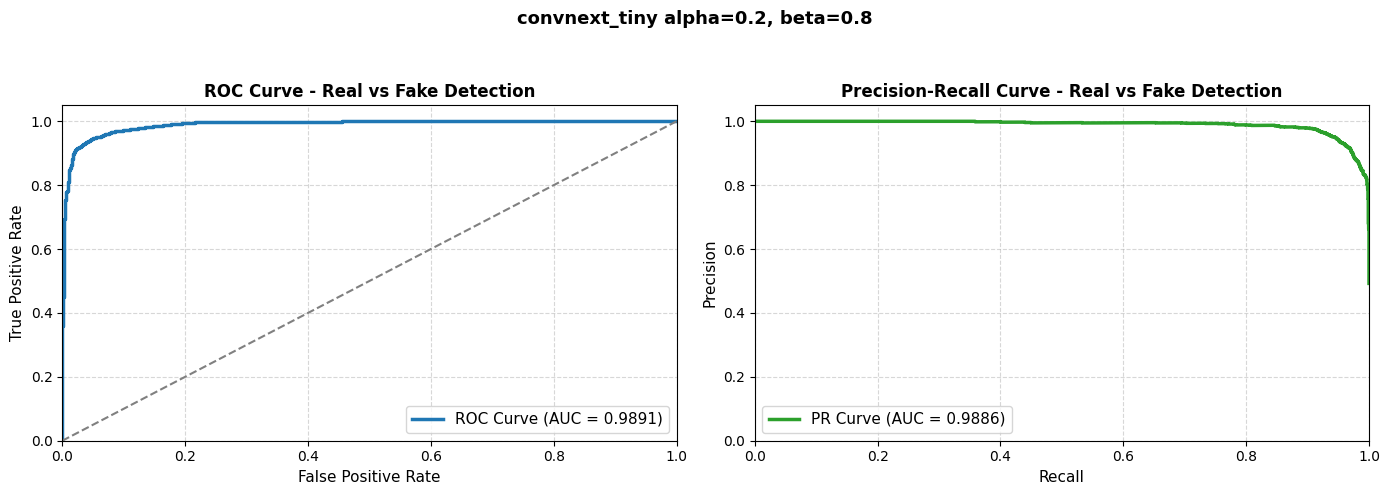
\includegraphics[height=5.1cm]{assets/roc_pr_curves.png}
\end{frame}

\begin{frame}{Robustness — Prediction Confidence}
  \footnotesize
  \begin{itemize}
    \item Prediction confidence is cleanly bimodal — almost nothing crosses the 0.5 threshold, indicating well-separated, well-calibrated predictions rather than borderline guessing.
  \end{itemize}

  \vspace{.3em}
  \centering
  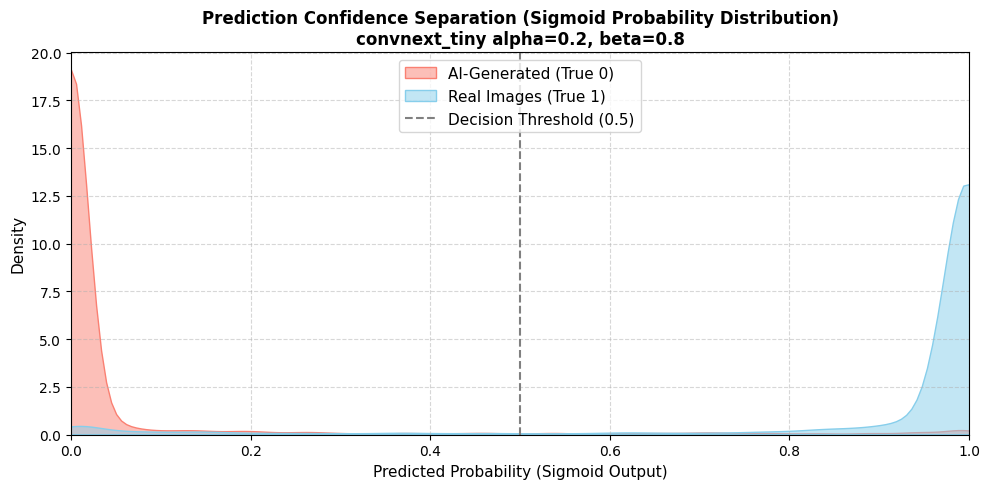
\includegraphics[height=5.1cm]{assets/prediction_distribution.png}
\end{frame}

\subsection{Interpretability}

\begin{frame}{What Is the Model Looking At?}
  \scriptsize
  \begin{itemize}
    \item GradCAM applied to \textbf{both} branches (spatial and frequency) for \textbf{both} heads: is a prediction driven by texture cues or by spectral artifacts?
    \item Spatial-branch heatmaps localize tightly on the main subject; frequency-branch heatmaps vary sample to sample rather than firing on a fixed region.
    \item Samples now drawn from a fixed (non-shuffled) validation order, so examples reproduce across runs.
  \end{itemize}

  \vspace{-.2em}
  \centering
  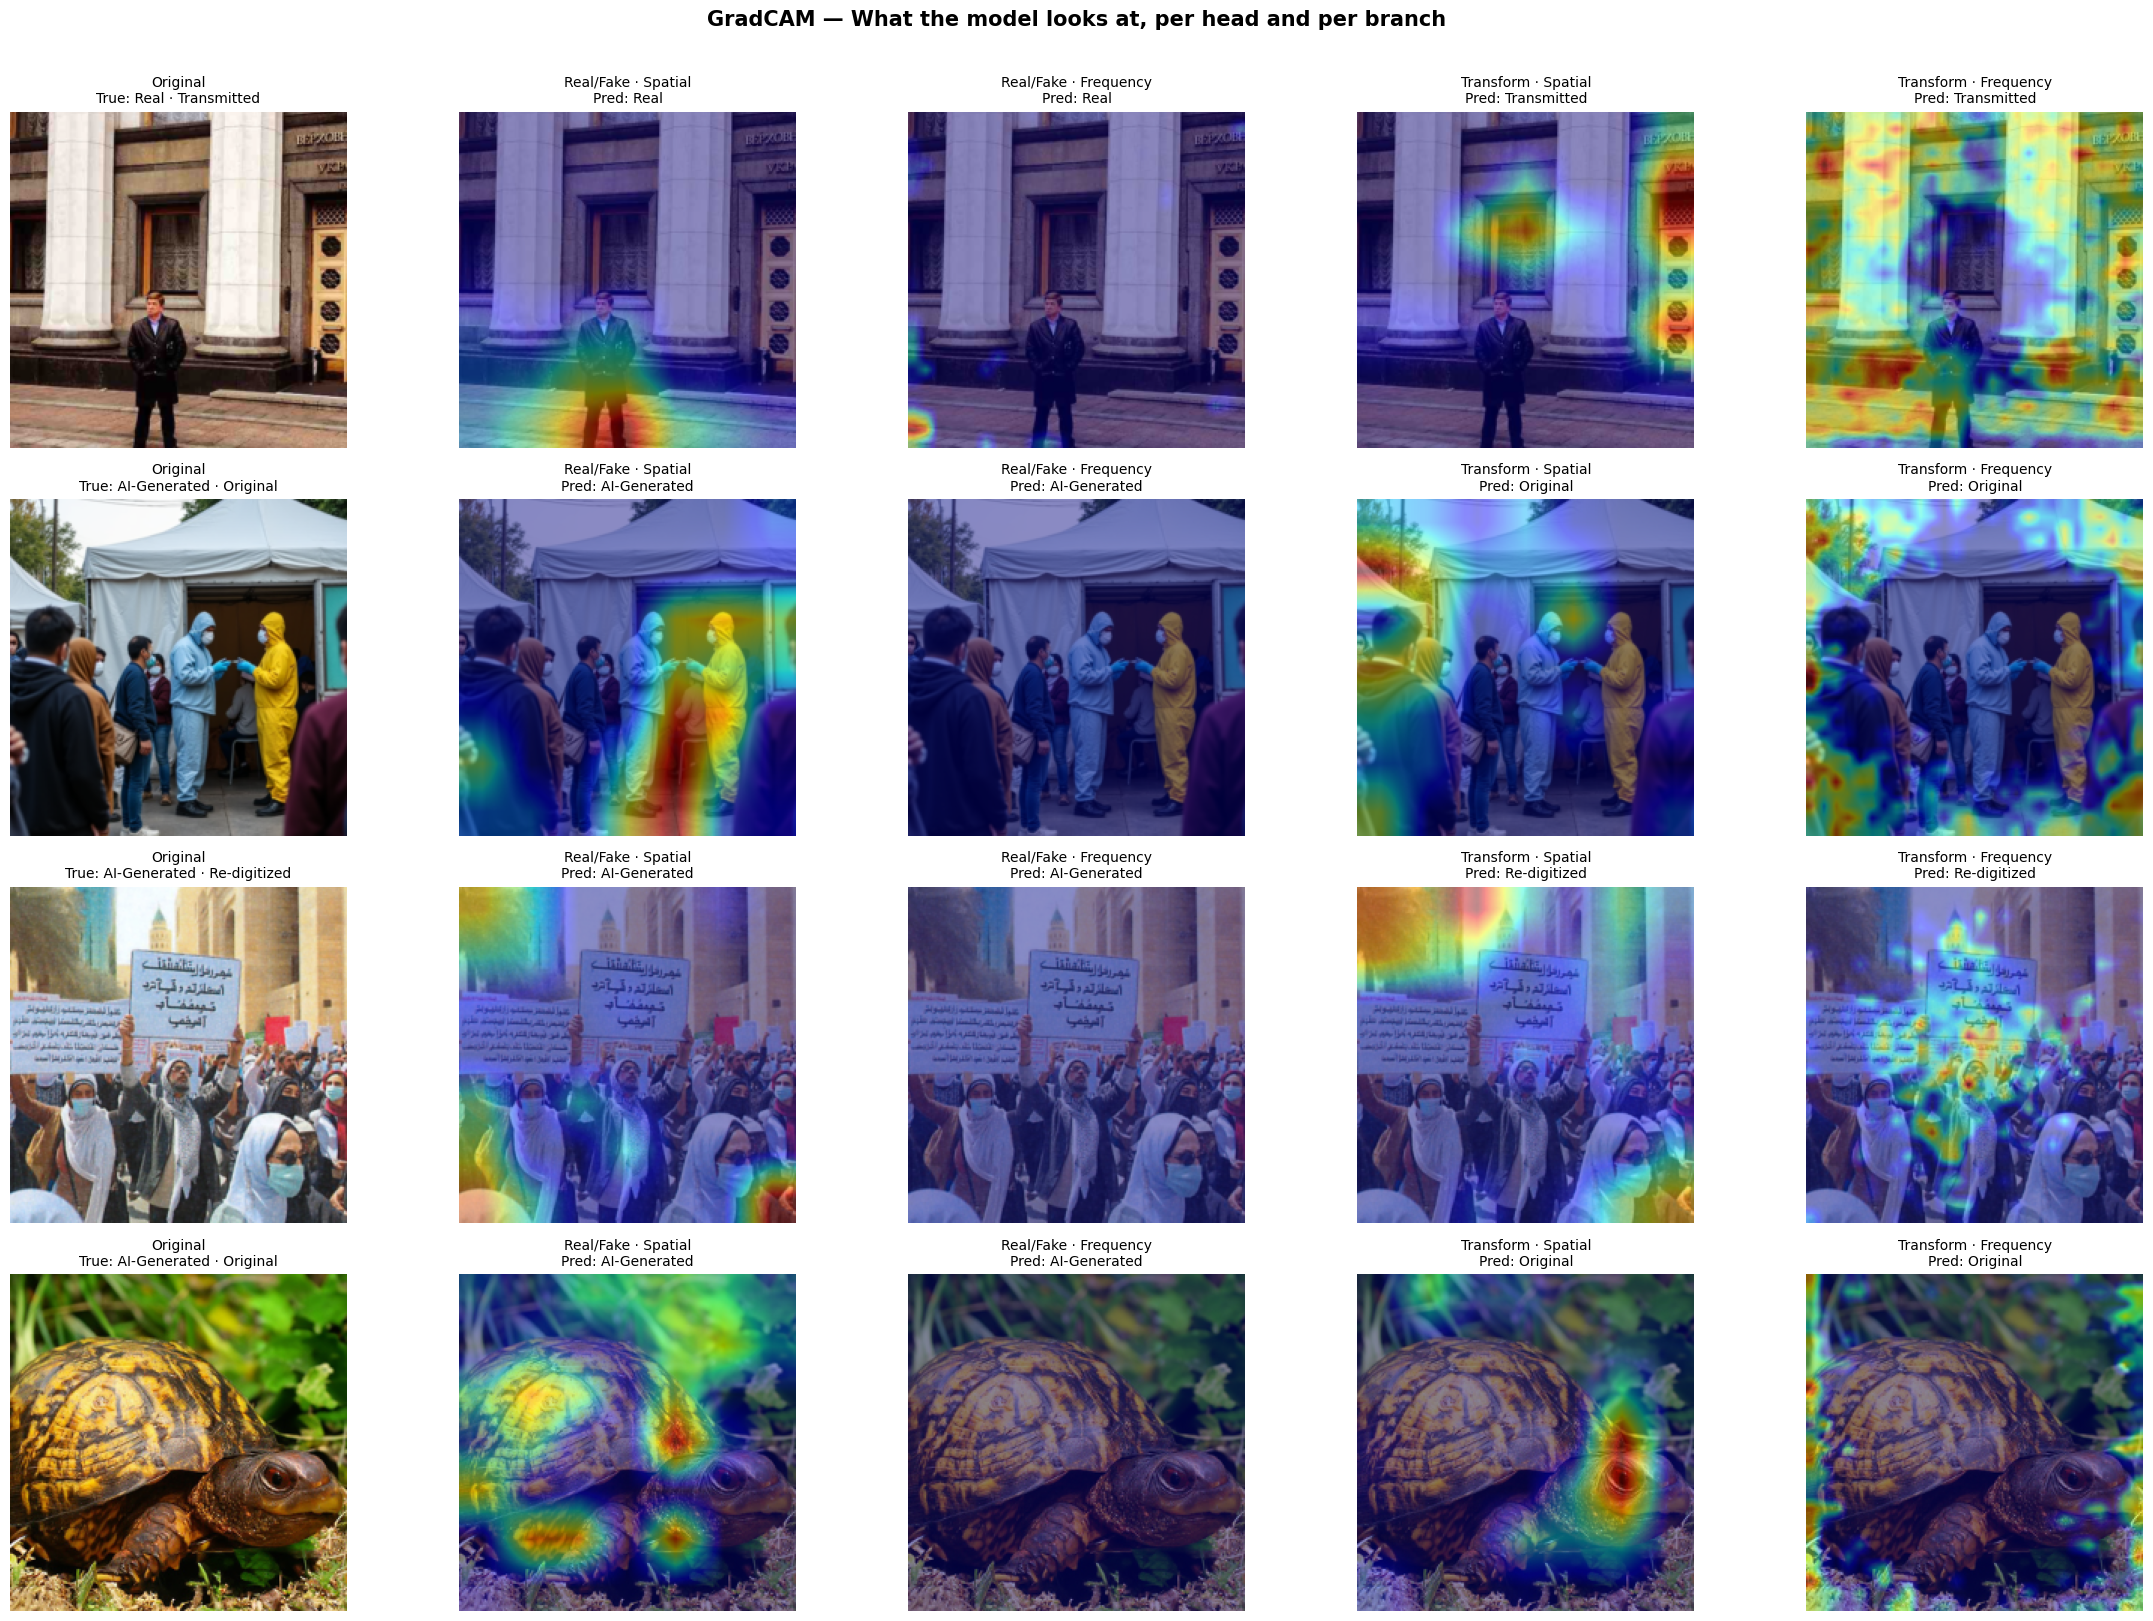
\includegraphics[height=4.6cm]{assets/gradcam.png}
\end{frame}

\section{Conclusions}

\begin{frame}{Conclusions \& Future Work}
  \footnotesize
  \begin{itemize}
    \item \textbf{Summary:} two-stream spatial+frequency fusion reaches 93.7--94.8\% RF accuracy, 92.2--94.4\% Transform accuracy, ROC-AUC $\geq$0.986 across two backbones.
    \item The $\alpha/\beta$ ablation confirms the multi-task design works: only the degenerate single-task extremes underperform; every balanced weighting does well on both tasks.
    \item Manual $\alpha/\beta$ tuning slightly edges out learned uncertainty weighting, which remains a solid no-search default.
    \item \textbf{Limitations \& future work:} single dataset, CNN/ConvNeXt only, no unseen-generator or per-branch-ablation testing — natural next steps.
  \end{itemize}
\end{frame}

\section{References}

\begin{frame}[allowframebreaks]{References}
  \footnotesize
  \printbibliography[heading=none]
\end{frame}


\end{document}
